%% For double-blind review submission, w/o CCS and ACM Reference (max submission space)
\documentclass[acmsmall,review]{acmart}\settopmatter{printfolios=true,printccs=false,printacmref=false}
%% \documentclass[acmsmall,anonymous,review]{acmart}\settopmatter{printfolios=true,printccs=false,printacmref=false}
%% For double-blind review submission, w/ CCS and ACM Reference
%\documentclass[sigplan,10pt,review,anonymous]{acmart}\settopmatter{printfolios=true}
%% For single-blind review submission, w/o CCS and ACM Reference (max submission space)
%\documentclass[sigplan,10pt,review]{acmart}\settopmatter{printfolios=true,printccs=false,printacmref=false}
%% For single-blind review submission, w/ CCS and ACM Reference
%\documentclass[sigplan,10pt,review]{acmart}\settopmatter{printfolios=true}
%% For final camera-ready submission, w/ required CCS and ACM Reference
%\documentclass[sigplan,10pt]{acmart}\settopmatter{}

%% Conference information
%% Supplied to authors by publisher for camera-ready submission;
%% use defaults for review submission.
\acmConference[PL'18]{ACM SIGPLAN Conference on Programming Languages}{January 01--03, 2018}{New York, NY, USA}
\acmYear{2018}
\acmISBN{} % \acmISBN{978-x-xxxx-xxxx-x/YY/MM}
\acmDOI{} % \acmDOI{10.1145/nnnnnnn.nnnnnnn}
\startPage{1}

%% Copyright information
%% Supplied to authors (based on authors' rights management selection;
%% see authors.acm.org) by publisher for camera-ready submission;
%% use 'none' for review submission.
\setcopyright{none}
%\setcopyright{acmcopyright}
%\setcopyright{acmlicensed}
%\setcopyright{rightsretained}
%\copyrightyear{2017}           %% If different from \acmYear

%% Bibliography style
\bibliographystyle{ACM-Reference-Format}
%% Citation style
%\citestyle{acmauthoryear}  %% For author/year citations
%\citestyle{acmnumeric}     %% For numeric citations
%\setcitestyle{nosort}      %% With 'acmnumeric', to disable automatic
                            %% sorting of references within a single citation;
                            %% e.g., \cite{Smith99,Carpenter05,Baker12}
                            %% rendered as [14,5,2] rather than [2,5,14].
%\setcitesyle{nocompress}   %% With 'acmnumeric', to disable automatic
                            %% compression of sequential references within a
                            %% single citation;
                            %% e.g., \cite{Baker12,Baker14,Baker16}
                            %% rendered as [2,3,4] rather than [2-4].


\usepackage{graphicx}
\usepackage{subfig}
\usepackage{caption}
%\usepackage{subcaption}
\usepackage[export]{adjustbox}

\begin{document}

\newcommand{\atomic}{\texttt{atomic}}
\newcommand{\asyncs}{async$*$}

\special{papersize=8.5in,11in}
\setlength{\pdfpageheight}{\paperheight}
\setlength{\pdfpagewidth}{\paperwidth}

% \titlebanner{Preprint.  Please do not redistribute}        % These are ignored unless
% \preprintfooter{Preprint.  Please do not redistribute}   % 'preprint' option specified.

\title{Measurement of Concurrency Patterns in Real-World Event Loop and Coroutine Code}
% \subtitle{\ldots and How to Make Cooperative Concurrency Safer with \texttt{atomic}}

%% Author information
%% Contents and number of authors suppressed with 'anonymous'.
%% Each author should be introduced by \author, followed by
%% \authornote (optional), \orcid (optional), \affiliation, and
%% \email.
%% An author may have multiple affiliations and/or emails; repeat the
%% appropriate command.
%% Many elements are not rendered, but should be provided for metadata
%% extraction tools.

%% Author with single affiliation.
\author{Benjamin Ylvisaker}
% \authornote{with author1 note}          %% \authornote is optional;
                                        %% can be repeated if necessary
% \orcid{nnnn-nnnn-nnnn-nnnn}             %% \orcid is optional
\affiliation{
  \position{Assistant Professor}
  \department{Department of Math and Computer Science}
  \institution{Colorado College}
  \streetaddress{14 E Cache La Poudre St}
  \city{Colorado Springs}
  \state{CO}
  \postcode{80903}
  \country{USA}
}
\email{bylvisaker@coloradocollege.edu}

\author{Clara Richter}
% \authornote{with author1 note}          %% \authornote is optional;
                                        %% can be repeated if necessary
% \orcid{nnnn-nnnn-nnnn-nnnn}             %% \orcid is optional
\affiliation{
  \institution{Colorado College}
}
\email{@coloradocollege.edu}

\author{Miguel Guerero}
% \authornote{with author1 note}          %% \authornote is optional;
                                        %% can be repeated if necessary
% \orcid{nnnn-nnnn-nnnn-nnnn}             %% \orcid is optional
\affiliation{
  \institution{Colorado College}
}
\email{@coloradocollege.edu}


\begin{abstract}

This paper is about atomicity in cooperative concurrency frameworks.
Cooperative concurrency frameworks like event loops, coroutines, async functions and cooperative threads are widely used for programming interactive systems like user interfaces and network clients.
Cooperative systems are much less prone to some kinds of concurrency bugs than preemptive threads, but not completely impervious.

Previous research has identified atomicity violations as one of the important kinds of concurrency defects that is possible in cooperative concurrency systems.
In this work we look at these atomicity violations from a couple different angles.
First we measure several popular web applications and find that conditions that are risky for atomicity violations are common.
Second we consider adding an atomic block to cooperatively concurrent languages.
We find a tricky, but resolvable semantic issue and measure implementation efficiencies enabled by atomic blocks.

%% This paper is about combining cooperative concurrency with atomic blocks.
%% In particular, we address two primary questions:
%% Why might this combination be useful?
%% What is tricky about making a clean semantics and implementation for languages that combine these concepts?

%%   The sophistication of multitasking in mainstream software has increased in recent years, thanks to the increasing richness of network communication, physical world interaction and multi-process software architectures.
%% These trends have pushed programming languages to offer better ways of writing such code.
%% As just one example of this trend, in recent years some flavor of coroutine has been standardized (or is heading towards standardization) in JavaScript, Swift, and C++.

%% This paper makes two primary contributions.
%% The first is an empirical study of multitasking in modern web applications.
%% Our primary finding is that in current practice, web JavaScript code tends to exhibit risky patterns, from the perspective of atomicity.
%% We argue that an \texttt{atomic} block primitive should be added to languages to help programmers avoid atomicity bugs.

%% We also experiment with two implementations of cooperative threads plus atomic: a JavaScript library and a dialect of C.
%% This investigation shows that this language design can be implemented in a flexible and efficient way.

\end{abstract}


%% 2012 ACM Computing Classification System (CSS) concepts
%% Generate at 'http://dl.acm.org/ccs/ccs.cfm'.
\begin{CCSXML}
<ccs2012>
<concept>
<concept_id>10011007.10011006.10011008</concept_id>
<concept_desc>Software and its engineering~General programming languages</concept_desc>
<concept_significance>500</concept_significance>
</concept>
<concept>
<concept_id>10003456.10003457.10003521.10003525</concept_id>
<concept_desc>Social and professional topics~History of programming languages</concept_desc>
<concept_significance>300</concept_significance>
</concept>
</ccs2012>
\end{CCSXML}

\ccsdesc[500]{Software and its engineering~General programming languages}
\ccsdesc[300]{Social and professional topics~History of programming languages}
%% End of generated code


%% Keywords
%% comma separated list
%% \keywords are mandatory in final camera-ready submission
\keywords{Cooperative concurrency, Multitasking, Atomicity}

\maketitle

% Outline:
% Introduction
%   Contributions
% Atomic or Interruptible?
%   On Atoms and Interrupts
%   Events
%   Cooperative Threads
%   Coroutines and Async Procedures}
%   What's Wrong with Threads?
% Activities
%   Shared Variables
%   Yield Insertion
%   Atomic
%   System Calls
%   Activities, Compared
% Implementation
%   Call Frame Allocation
%     Contiguous Allocation
%     Individual Heap Allocation
%     Split/Segmented Stacks
%     Dynamic Contiguous Stacks
%     Hot Stacking
%   Yield Implementation
%     Yield in Atomic Mode
%     Function Pointers
%     Yields
%   Asynchronous System Calls
%   Translation
%   Activities in JavaScript
% Evaluation
%   Building an App with Activities
%   Task Memory Overhead
%   Task Spawn and Switching Speed
%   Just Calling
%   Yielding
%   Microbenchmark Summary
% Related Work
%   Other Multitasking Abstractions
% Summary and Discussion



\section{Introduction}

Many applications are highly multitasked.
They have lots of balls in the air at the same time: network communication, queries to databases, multiple I/O modalities to monitor and manage.
Applications use a wide range of language and core library features to implement multitasking: threads, event loops, coroutines, async functions, functional reactive programming, etc.\footnotemark{}

\footnotetext{Some of these features are also relevant to \emph{parallelism} (i.e. physical simultaneity), but parallelism is \emph{not} the subject of this paper or the project it describes.}

Many popular application programming frameworks use some form of \emph{cooperative} multitasking, because of the fear that \emph{preemption} too easily causes concurrency bugs.
In particular, in cooperative models the minimum granularity of atomicity is much larger, which dramatically reduces the likelihood of some kinds of concurrency problems.
While the authors of this paper are sympathetic with this line of reasoning, we remind the reader that cooperativeness does not completely eliminate the risk of concurrency defects\footnotemark{}.
In fact, there has been much research in the last decade on cataloging, exposing, diagnosing and fixing concurrency bugs in web and mobile applications that use cooperative concurrency.

\footnotetext{This is similar to how garbage collection reduces, but does not eliminate, exposure to memory bugs \cite{Grossman2007}.}

One of the most important categories of defects identified by this research is atomicity violations.
In the broadest interpretation, atomicity violations occur when a programmer writes some logic that assumes two (or more) actions will be performed by a particular task without interruption, but another task does in fact perform a conflicting action in the middle of the intended atomic actions.
In the simplest case, the actions can be local memory operations, but they can also be interactions with databases, networks or user interface elements.

Systems for enforcing atomicity are widely used.
Atomic transactions are nearly universal in databases, where they ensure that multiple reads and writes are performed without interruption.
Herlihy and Moss \cite{Herlihy1993} kicked off decades of research on bringing this idea to general purpose multithreading languages in the form of a block that can make an arbitrary sequence of statements appear atomic.

% Transactions are a classic concept in databases and distributed systems. Transactional support in hardware [30], programminging languages [21], and libraries [45] had early advocates, with recent interest beginning with Harris and Fraser’s work for Java [24]. Approaches to implementing TM in compilers [2, 25, 26, 27, 32, 36, 44, 46], libraries [29, 37, 28], hardware [23, 9, 38, 42, 4, 40, 41], and software/hardware hybrids [12, 34] have been published, and transactions are part of several next-generation languages [3, 10, 11].

% XXX , because of challenges with implementation efficiency and semantic trickines with concurrent access to resources from atomic blocks and non-atomic code

The idea of \emph{preemptive} multithreading languages with atomic blocks is compelling (just a small sample: \cite{Harris2003, Harris2005, Ringenburg2005, Herlihy2006, Ni2008}), but has seen relatively little use outside of research labs because of technical challenges.
The main question this paper addresses is: Is it a good idea to combine atomic blocks with \emph{cooperative} concurrency models, like event loops or cooperative threads?
We primarily focus on three sub-questions:
\begin{enumerate}
\item Do atomic blocks bring software engineering benefits to cooperative concurrency?
\item Are there any semantic or language design problems with this combination?
\item Are there interesting implementation efficiency issues raised by this combination?
\end{enumerate}

We gather evidence for an affirmative answer to the first question by measuring widely used web applications\footnotemark{}.
We observe that risky patterns are common.
In particular, there are many short-duration chains of continuations.
It would be easy for such code to pass testing, even though it is possible for conflicting tasks to execute in gaps between continuations.
One way to increase the safety of such chains is with a language-level atomic block.

\footnotetext{We study web applications for the simple reason that a large amount of presumably highly vetted code is easily available for the studying.}

In investigating the second question, we noticed the following tension between atomic blocks and cooperative concurrency:
\begin{enumerate}
\item There are multiple reasonable definitions for the nesting of atomic blocks and task spawns; no interpretation works well in all contexts.
\item Many cooperative concurrency frameworks are \emph{anonymous} in the sense that they lack an explicit notion of task identity.
  Anonymity makes it hard for the system to know whether the programmer intended an asynchronous continuation to be logically a single interruptible task, or a new concurrent task.
  This uncertainty further compounds point 1, because spawns cannot be distinguished unambiguously from task continuations.
\end{enumerate}
To the best of our knowledge, this is a novel observation.
This implies that \emph{if} a cooperative multitasking framework is to include atomic blocks, it should have explicit task identities (i.e. some flavor of cooperative multithreading).

To investigate the third question, we implemented cooperative threads with atomic blocks in two contexts: as a library built on top of JavaScript's coroutines (\texttt{function*}) and \texttt{Promises}, and as a dialect of C.
We observe that such a library can be used with little change relative to popular JavaScript patterns, and that it mostly integrates well with legacy code.
In the C dialect implementation we discover a new call frame allocation strategy -- enabled by atomic blocks -- that combines the speed of contiguous frame allocation with the memory efficiency of individual linked frame allocation.

In summary, the contributions of this paper are:
\begin{itemize}
\item A measurement study of multitasking in web applications.
\item An analysis of the tension between atomic blocks and anonymous multitasking.
\item An exploration of integrating cooperative threading with atomic blocks in an existing multitasking ecosystem.
\item A new call frame allocation strategy for languages with atomic blocks.
\end{itemize}

All code and data described in this paper is available publicly on GitHub [URL removed for blind review].

\section{Multitasking in Web JavaScript}

We begin with a brief (and incomplete) history of multitasking in JavaScript.
In the beginning, the designers of JavaScript decided not to include preemptive threads, because they caused an unacceptably high risk of concurrency bugs.
One good entry into the vast literature on the difficulties of diagnosing and fixing multithreading defects is \cite{Lu2008}.
These challenges have long been understood; more than two decades ago Ousterhout wrote a popular critique of threads \cite{Ousterhout1996}.

\begin{figure}
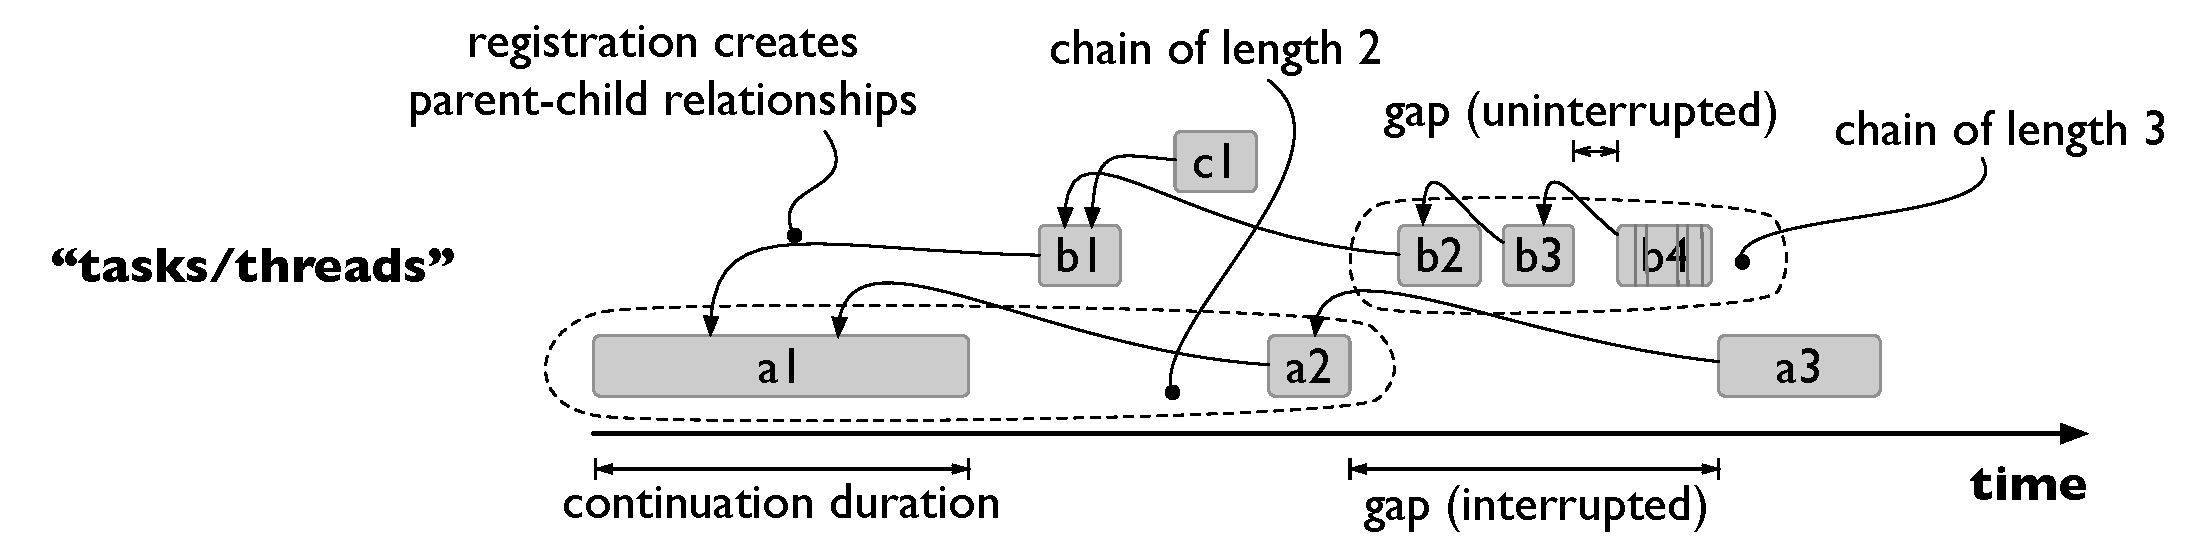
\includegraphics[width=0.99\textwidth]{Figures/continuation_tree}
\caption{The features of JavaScript event execution that our modified Chromium browser measures.
  The gray boxes are continuations.
  The continuations are arranged in rows to suggest that they belong to the same task.
  However, event loop systems do not have this concept, so this is purely an intuitive interpretation.
  For example, \textsf{a2} and \textsf{b1} are both children of \textsf{a1}, and there is no way for the system to know what logical task either belongs to.}
\label{fig:continuation_tree}
\end{figure}

Early versions of JavaScript supported only event-based concurrency.
The simple picture of the implementation of JavaScript is that there is a single event dispatcher that stores a collection of functions waiting for some enabling condition.
These functions can be registered by primitive APIs, like \texttt{setTimeout}.
In all cases we refer to such registered functions as \emph{continuations}.
We refer to a continuation plus its enabling condition as an \emph{event}.
When an event's condition is satisfied, the dispatcher may execute its continuation.

Simple event programming has some serious drawbacks.
For example, management of resources whose lifetime spans multiple events and propagation of errors can be tricky.
This leads to a style of programming referred to as \emph{stack ripping} \cite{Adya2002}, or more colloquially \emph{callback hell}.
These and more subtle problems are well analyzed and criticized by von Behren et al. in \cite{Behren2003a}.

The increasingly sophisticated multitasking in modern applications and the well-known problems with threads and events have increased the use of alternatives in recent years, the most popular of which are \emph{coroutines} and \emph{async procedures}.
Examples include async/await, added to C\#/.Net in 2012; function generators (\texttt{function*}, essentially coroutines), added to JavaScript with ECMAScript 6 (standard published in 2015); even the staid C++ community is considering adding native support for coroutines (currently on the short list for inclusion in the C++20 standard).
Coroutine implementations are not \emph{new}; for example, Modula-2 had coroutines in the 1980s and several ``scripting'' languages (Ruby, Python, Lua) added support in the early aughts.
However, coroutines and async functions were not widely used in application programming until relatively recently.

The most recent versions of JavaScript have native support for promises, coroutines and async functions.
Promises complicate JavaScript's event dispatcher semantics somewhat.
Promises can be chained through their \texttt{then} method.
Continuations registered via a \texttt{Promise}'s \texttt{then} method are treated differently from ``normal'' continuations.
Promise resolutions are considered ``microtasks''.
Microtasks in a sense take precedence over regular tasks; as long as the microtask queue is not empty, regular task execution will be delayed indefinitely.

A style of programming that mixes async functions and \texttt{Promise} chaining has become popular in JavaScript communities.
This style of programming makes multitasking much more convenient than programming with explicit callbacks.
This evolution in style has made it feasible for more developers to write more highly multitasked applications.

\subsection{Measurements}

The theme of the measurements in the remainder of this section is: perhaps there are ways in which it is now too easy to write highly asynchronous code.
In particular, the concurrency safety of JavaScript and similar languages has always relied heavily on the atomicity of relatively long-running functions (long-running relative to the microscopic processor clock rate scale).
As programmers chop applications up into chains of smaller functions, atomicity problems reemerge as an interesting risk.
We do \emph{not} show any specific atomicity violations in this paper.
Rather, the measurements demonstrate that conditions that make atomicity violations possible are empirically common.

We modified a version of Chromium to gather data on JavaScript behavior from web applications.
Figure \ref{fig:continuation_tree} illustrates the features of JavaScript execution that our modified browser measures:

\begin{itemize}
\item Continuation duration is the time difference between when the dispatcher passes control to a continuation and when it returns.
\item We measure both the duration and number of microtasks in microtask batches.
  More on microtasks below.
  (The vertical lines in continuation \textsf{b4} in the Figure are meant to suggest individual microtasks within a batch.)
\item Parent-child relationships are inferred by recording which continuation (the parent) is running when potential children are registered; this relation is referred to as \emph{async-contexts} in \cite{Loring2017}.
  There is actually a more subtle distinction between what that paper refers to as \emph{linking contexts} and \emph{causal contexts} when dealing with Promises.
  We primarily analyze raw callbacks, for which this distinction does not exist.
\item A \emph{gap} is the time difference between the start of a continuation and the end of its parent.
  A gap is \emph{interrupted} if \emph{any} other continuation runs between parent and child.
\item Figure \ref{fig:continuation_tree} suggests an intuitive notion of tasks, where a continuation can either be a logical continuation of its parent's task or a newly spawned concurrent task.
  This concept is sufficiently important that several libraries and tools have related ideas, like Zones in AngularJS, Async Hooks in Node.js and Async Call Stacks in the Chrome Developer Tools.
  Unfortunately, it is not part of standard JavaScript, so in general it is not possible to automatically and precisely infer.
\end{itemize}

% Async Hooks. 2016. https://github.com/nodejs/diagnostics/tree/ master/tracing/AsyncWrap.
% Async Call Stacks. 2014. http://www.html5rocks.com/en/tutorials/developertools/async-call-stack/.
% [26] Zones. 2014. https://github.com/angular/zone.js.

\begin{figure}
    \centering
    \begin{minipage}[t]{0.47\textwidth}
        \centering
        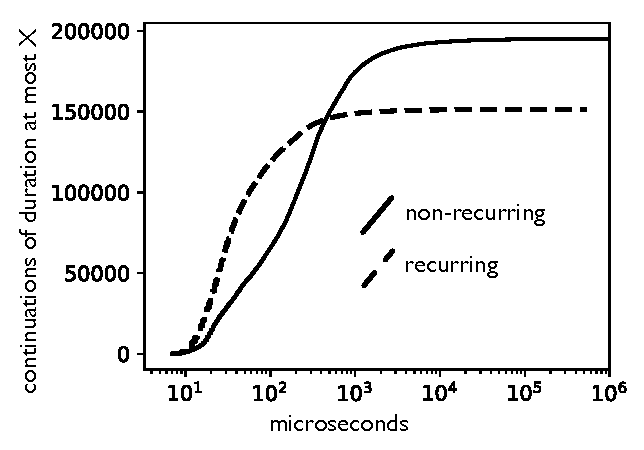
\includegraphics[width=1.0\textwidth]{Graphs/durations_bw}
        \caption{Most continuations are short.
  Many are very short.}
        \label{fig:graph_duration}
    \end{minipage}\hfill
    \begin{minipage}[t]{0.47\textwidth}
        \centering
        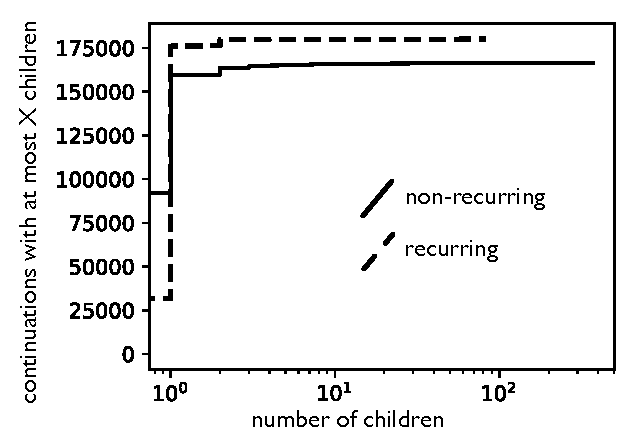
\includegraphics[width=1.0\textwidth]{Graphs/branching_bw}
        \caption{Most continuations have one child.
A few have many, many children.}
        \label{fig:graph_branching}
    \end{minipage}
\end{figure}

\subsubsection{Duration}

Our first observation from Figure \ref{fig:graph_duration} is that most continuations are short.
A large majority take less than one millisecond, and many are much shorter.
(This figure combines the data for both microtask batches and normal tasks.)

Short continuations are the first risky condition for atomicity violations.
Longer continuations would naturally lead to longer-duration chains of continuations.
All other things being equal, it is easier for programmers to miss atomicity problems in shorter chains.
Also, it is interesting to see that JavaScript programmers seem to overwhelmingly abide by the norm that continuations should complete quickly, in order to keep applications responsive.
This observation will be important when we discuss API design later.

The difference between the solid and dashed lines in Figure \ref{fig:graph_duration} highlights the importance of recurring events.
In JavaScript, certain APIs, like \texttt{setInterval} and \texttt{XMLHttpRequest} register continuations that the event dispatcher can call multiple times.
As you can see, these recurring continuations account for a majority of the shortest.
(A majority of those are accounted for by status updates on downloading files.)
However, even among the non-recurring continuations, there are still quite a few towards the short end of the distribution.
In several of the measurements and analyses below we \emph{filter out the recurring events}, because they are less relevant to our focus on chains of continuations that could be mistaken for being atomic.

\subsubsection{Branching and Concurrency}

Next, notice in Figure \ref{fig:graph_branching} that most continuations have \emph{at most} one child.
Among recurring continuations there are more with one child; among non-recurring continuations there are more with zero.
The fact that there are many single-child continuations suggests that JavaScript programmers are breaking linear sequences of logic up into multiple continuations.
Presumably they are doing this either intentionally to improve responsiveness, or because of libraries that only offer an async interface.
Otherwise, why not combine these continuations into a single function?

Though most continuations have few children, a few continuations have many.
This can be seen in the long tails in Figure \ref{fig:graph_branching}.
(There are at least a few continuations with hundreds of children!)
A consequence of this branching is that the continuation trees we studied exhibit quite a lot of concurrency.
For each continuation we define its degree of concurrency to be the number of continuations that \emph{will} run \emph{after} it, but were registered before it started.
In other words, how many parent-child edges are ``live'' across each continuation?

Figure \ref{fig:graph_concurrency} shows the results of our concurrency measurements.
Notice that most continuations are concurrent with at least 10 edges, and a substantial minority are concurrent with at least 100.
This high degree of concurrency is our second risky condition for atomicity violations.
If most continuations had a low degree of concurrency, there would be little opportunity for a concurrent task to perform a conflicting action.

\begin{figure}
    \centering
    \begin{minipage}[t]{0.47\textwidth}
        \centering
        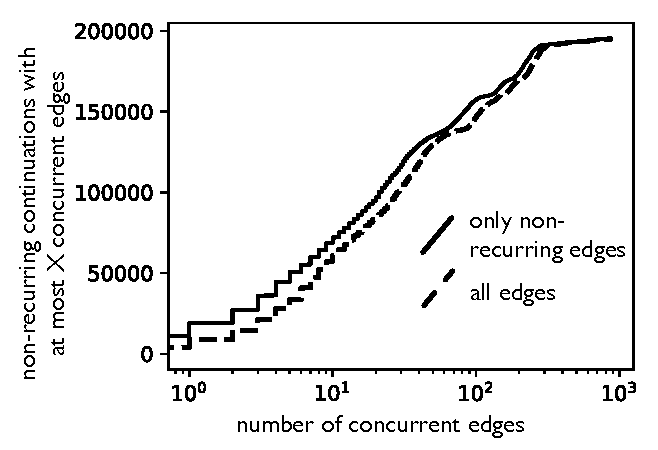
\includegraphics[width=1.0\textwidth]{Graphs/concurrency_bw}
        \caption{Most continuations are concurrent with several parent-child edges.
        In this graph we only include non-recurring continuations.}
        \label{fig:graph_concurrency}
    \end{minipage}\hfill
    \begin{minipage}[t]{0.47\textwidth}
        \centering
        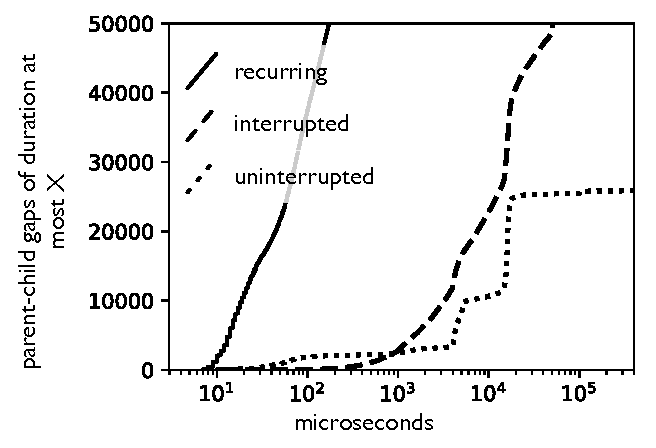
\includegraphics[width=1.0\textwidth]{Graphs/gaps_bw}
        \caption{
          Most gaps are of reasonable length, but a nontrivial percentage are quite short.
          This graph is truncated at half a second because we are not interested in long gaps.
          This graph is also truncated at 50,000 because we are less interested in the gaps before recurring events.}
        \label{fig:graph_gaps}
    \end{minipage}
\end{figure}

\subsubsection{Gaps and Chains}

The last basic measurements of continuation trees that we consider are the lengths of parent-child gaps and short chains.
Figure \ref{fig:graph_gaps} shows that many gaps are quite short.
The majority of the shortest gaps are between recurring events, which are less interesting to us.
However, there are still quite a few gaps between non-recurring events that are shorter than 10 milliseconds.

A particularly interesting feature to notice is that there are thousands of uninterrupted gaps in the 100s of microseconds range, but far fewer interrupted gaps.
This means that interruption of gaps of that size is possible, but rare.
This combination is bad for atomicity violation risk.
If interruption of gaps shorter than some limit were impossible, such gaps would clearly represent no atomicity violation risk.
In interruption were common, it would be more likely that testing would catch possible atomicity violations.

Figure \ref{fig:graph_chains} shows the duration of continuation chains of length 2, 3 and 4 (that is, the time difference between the beginning of first continuation in the chain and the end of the last).
For this graph we filtered out all chains with recurring continuations.
This data is not surprising based on the continuation duration and gap data and presented above.
We see that while many chains are of a fairly reasonable duration (say, dozens to hundreds of milliseconds), there is a non-trivial fraction under 10 milliseconds, and even some under 1 millisecond.

\begin{figure}
    \centering
    \begin{minipage}[t]{0.47\textwidth}
        \centering
        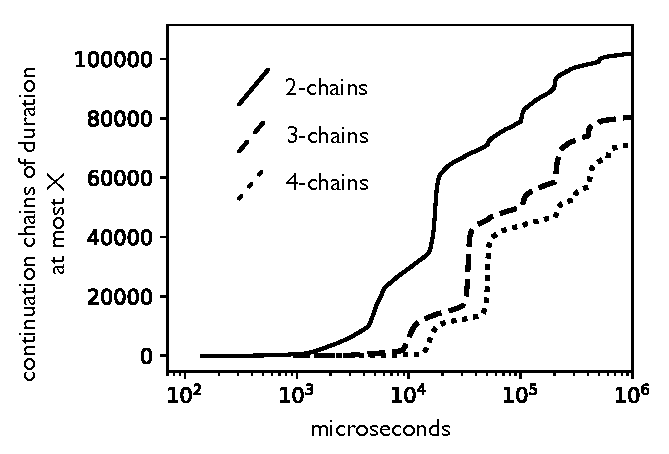
\includegraphics[width=1.0\textwidth]{Graphs/chains_bw}
        \caption{Most chains of continuations are reasonably long.
        However, some are quite short; a nontrivial minority are under 10ms.}
        \label{fig:graph_chains}
    \end{minipage}\hfill
    \begin{minipage}[t]{0.47\textwidth}
        \centering
        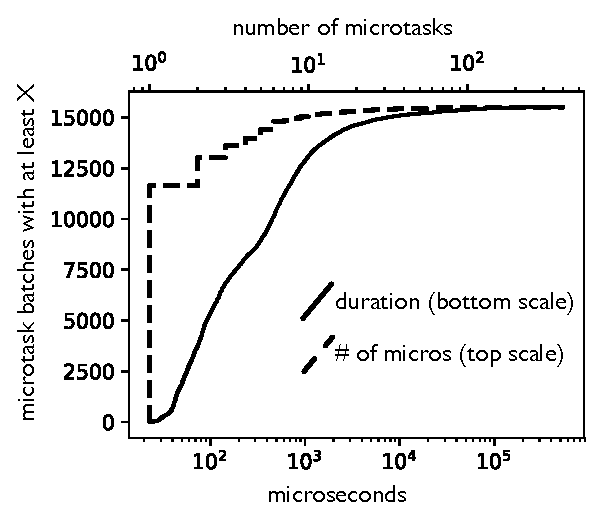
\includegraphics[width=1.0\textwidth]{micros_graph_bw}
        \caption{Most microtask batches are short, but a nontrivial number are long enough to possibly exceed the time and/or microtask count limits of some reasonable implementations.}
        \label{fig:graph_microtasks}
    \end{minipage}
\end{figure}

\subsubsection{Microtasks}

In this subsection, we look at microtasks, which are tangential to the main plot of this paper, but still somewhat interesting.
Microtasks are a special subset of events in JavaScript; the most common source of microtasks is \texttt{Promise} resolution.
Unlike regular events, as soon as at least one microtask is registered, the dispatcher switches to running microtasks.
During the execution of a microtask, more microtasks can be registered, and the dispatcher will not run another normal (non-microtask) event until the microtask queue is empty.

Figure \ref{fig:graph_microtasks} shows data about the durations and microtask counts of microtask batches.
Most batches are fairly short/small by both metrics, which seems good.
However, a nontrivial minority of microtask batches get into the 10s and even 100s of milliseconds and/or dozens or hundred of microtasks.
At that size, these microtask batches start to be potential responsiveness problems.
When batches of microtasks get too long, programmers may make ad hoc decisions about where to break them up, thus creating more opportunities for atomicity problems.

\subsubsection{Atomic Can Cause Unresponsiveness}

One interesting metric that we were \emph{not} able to derive from our continuation trees is the variance in durations of dynamic instances of specific source-level chains of continuations.
This is an interesting metric because it is evidence for how likely it is that using a source-level atomic block would increase risks to responsiveness.
To be concrete, imagine a block of source code that generates a chain of continuations that is usually very short, but is occasionally long.
If such a block of source was wrapped in atomic it could create a responsiveness problem in those occasional situations.
The reason this metric is hard to measure on popular websites is that most of them seem to deploy JavaScript code that has been compiled (e.g. by Babel, Google Closure, or from some other language entirely) and uses frameworks (like Angular or Relay).
One of the consequences of this is that often there are shim functions around continuation registration and/or dispatching, which makes it hard to infer source-level information from dynamic traces.

\subsection{Instrumentation and Data Source Details}

To gather the traces for our continuation trees we inserted instrumentation in two sections of Chromium: The CoreProbes code in the WebKit tree and the isolate and execution code in the V8 tree.
The former gives us information about the registration and execution of normal events.
The latter gives is information about microtasks and the execution of JavaScript functions.

We gathered traces from several dozen of most popular English-language websites according to Wikipedia's list.
For each site we gathered a small number of traces while performing simple actions like logging in, searching, or posting to a discussion.
So far we have only performed coarse aggregate analyses; we have not attempted to find differences between different sites, libraries, or coding styles.

\subsection{Is This Actually a Problem?}

In this paper we do not present any specific atomicity violations, only evidence that risky patterns are common.
This leads to a couple important questions:
How confident can we be that the patterns we studied are associated with real atomicity defects, and are thus worth doing something about?
If these patterns are a valid concern (of any magnitude), what explains their existence in the most widely used web applications?
We will address the second question first.

\subsubsection{An Explanation for the Rise of Short Chains}

There is always a dilemma in cooperative concurrency associated with the durations of whatever the atomic chunks are.
The longer the chunks, the greater the risk to responsiveness, appearing jittery, or missing I/O deadlines.
The shorter the chunks, the greater the risk of a programmer splitting some logic that should be atomic into multiple chunks.

This dilemma is particularly acute when designing library interfaces, because libraries should work well in multiple specific contexts; quite often those contexts are unknown to the library authors.
To be more concrete, when library authors design APIs, they face the choice between making a call atomic or async in some way (callback, Promise, async method, whatever).
In some cases this choice is easy.
If a function always completes quickly, then it should be atomic.
If a function usually takes a long time, then it should be async.

Unfortunately, many functions fall in the awkward middle territory, where some calls are quick and others are not.
For these functions, async is in some sense the easier choice, because long-running atomic calls create immediately obvious responsiveness problems that cannot be easily worked around by applications.
On the other hand, atomicity problems are not as obvious and in principle can be worked around with application-level synchronization.

A similar line of reasoning led the developer's of Microsoft Windows' core Windows Runtime (WinRT) library to replace many atomic procedures with asynchronous ones in Windows 8.
In a post on the Microsoft Developer Blog \cite{Windows8Team2012}, the team explains that they did this for procedures that ``could likely take longer than 50 milliseconds to execute''.

In some recently defined JavaScript APIs, even some functions that will execute quickly in most reasonable contexts have an async interface.
As one example among many, the PBKDF2 key derivation function in the WebCrypto library returns a Promise.
PBKDF2 is a function that takes a number of iterations as a parameter.
On a modern computer the PBKDF2 function takes in the rough neighborhood of one microsecond per iteration.
So the iteration parameter must be set very high for this function to represent a responsiveness problem.
In contexts where the iteration count is lower, an atomic interface would be preferable.

Consider a more extreme example: sending a network request.
Sending a message over a wide area network will inevitably be slow, and network operations are generally defined to be asynchronous to accommodate this.
However, in a microservices software architecture, applications use network protocols to communicate with other processes that might be running on the same computer.
Depending on the details of a specific request to a peer process, it may actually be fast enough that the requester would prefer to block while waiting for the response.

These examples illustrate what we believe is a general trend towards applications using libraries with async interfaces.
The data presented in the previous section is consistent with this now being common practice.

% SPAs, end-to-end encryption

\subsubsection{The Atomicity Violation Struggle is Real}

There has been a great deal of research on atomicity violations in general \cite{Lu2008}.
More directly relevant to this paper, several researchers have worked on detecting and classifying concurrency bugs in event-driven web and mobile applications \cite{Petrov2012, Hsiao2014, Mutlu2015, Zhang2017}.
These papers focus on ``races'', which are related to atomicity violations.
Every atomicity violation involves a race, in some sense, but not every race is part of an atomicity violation.

% Petrov2012  Race Detection for Web Applications
% Hsiao2014  Race Detection for Event-driven Mobile Applications
% Mutlu2015  Detecting JavaScript Races That Matter
% Zhang2017  RClassify: Classifying Race Conditions in Web Applications via Deterministic Replay
% XXX Shin Hong, Yongbae Park, and Moonzoo Kim. Detecting concurrency errors in client-side java script web applications. In IEEE International Conference on Software Testing, Verification and Validation, pages 61– 70, 2014.

Another kind of evidence is analysis of concurrency bugs in JavaScript applications based on real bug databases \cite{Davis2017, Hong2014, Wang2017}.
The authors of \cite{Davis2017} reported that 69\% of the 16 concurrency bugs they studied involved an atomicity violation, while the authors of \cite{Wang2017} reported 65\% of 57 bugs.
The latter paper goes on to report that of the atomicity violation bugs, 27\% were fixed by adding synchronization or switching to an atomic API.
These papers specifically looked at applications based on Node.js, which is somewhat different from browser JavaScript.
However, with the rising popularity of tools like Webpack, Browserify and Gulp, libraries from the expansive NPM ecosystem are increasingly being used in code written for browsers\footnotemark{}.
This means that the differences between browser JavaScript and Node.js JavaScript are shrinking.
This phenomenon even has a name: Isomorphic JavaScript \cite{Brehm2013}.
Also while Node.js has traditionally been used to develop servers, it is increasingly being used in desktop and mobile apps via tools like Electron, Cordova and Ionic.

\footnotetext{One remarkable metric of this part of the JS ecosystem is that the NPM package repository had over 600,000 modules, as of March, 2018 \cite{ModuleCounts}.}

\begin{figure}
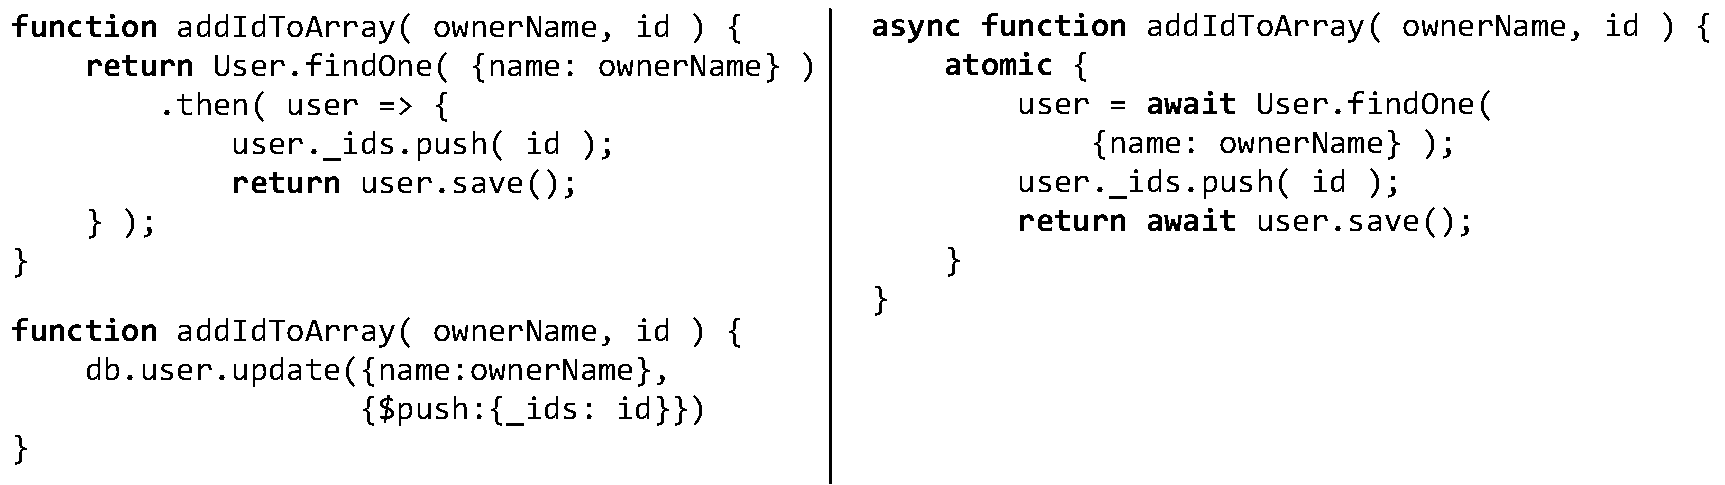
\includegraphics[width=0.97\textwidth]{Code/atomicity_violation}
\caption{An example of an atomicity violation from a real application, adapted from \cite{Wang2017}.
  The top left is the original buggy code.
  The key is that there are two database API calls (\texttt{findOne} and \texttt{save}); if the DB state changes between these two, it can be corrupted.
  The bottom left is how the actual developers fixed the problem.
  They replaced the two API calls with a single atomic call that has the same effect.
  The right side is how the bug could be fixed in a hypothetical variant of JavaScript with atomic blocks.}
\label{fig:atomicity_violation}
\end{figure}



% Davis2017 11/16 atomicity violations
% Wang2017  65% atomicity violations --> 27% fixed by adding synchronization or switching to an atomic API

\subsubsection{Potential Solutions}

The remainder of this paper explores atomic blocks as a mitigation for atomicity problems.
However, there are other viable strategies that programmers are surely already using to some extent.

One strategy is to use a ``functional'' style of programming, with immutable data structures and application-level atomic transactions.
If this style is used consistently, then it is unimportant how small the atomic chunks are; the likelihood of concurrency bugs depends very little on scheduling.

Even if code is written in the more common imperative style, careful software engineering can still protect against atomicity violations.
For example, programmers can use an adversarial scheduler to flush out concurrency bugs.

While the authors of this paper gladly endorse these strategies, we observe that quite a few applications are written with a modest level of software engineering care.
It would be nice if there was a simple tool (like an atomic block) that could help avoid at least some concurrency issues.
Also a note of caution: some techniques are appropriate for maintaining atomicity within the bounds of a single process, but are less relevant when I/O is involved.

\section{The Tension Between Anonymous Multitasking and Atomic}

\begin{figure}
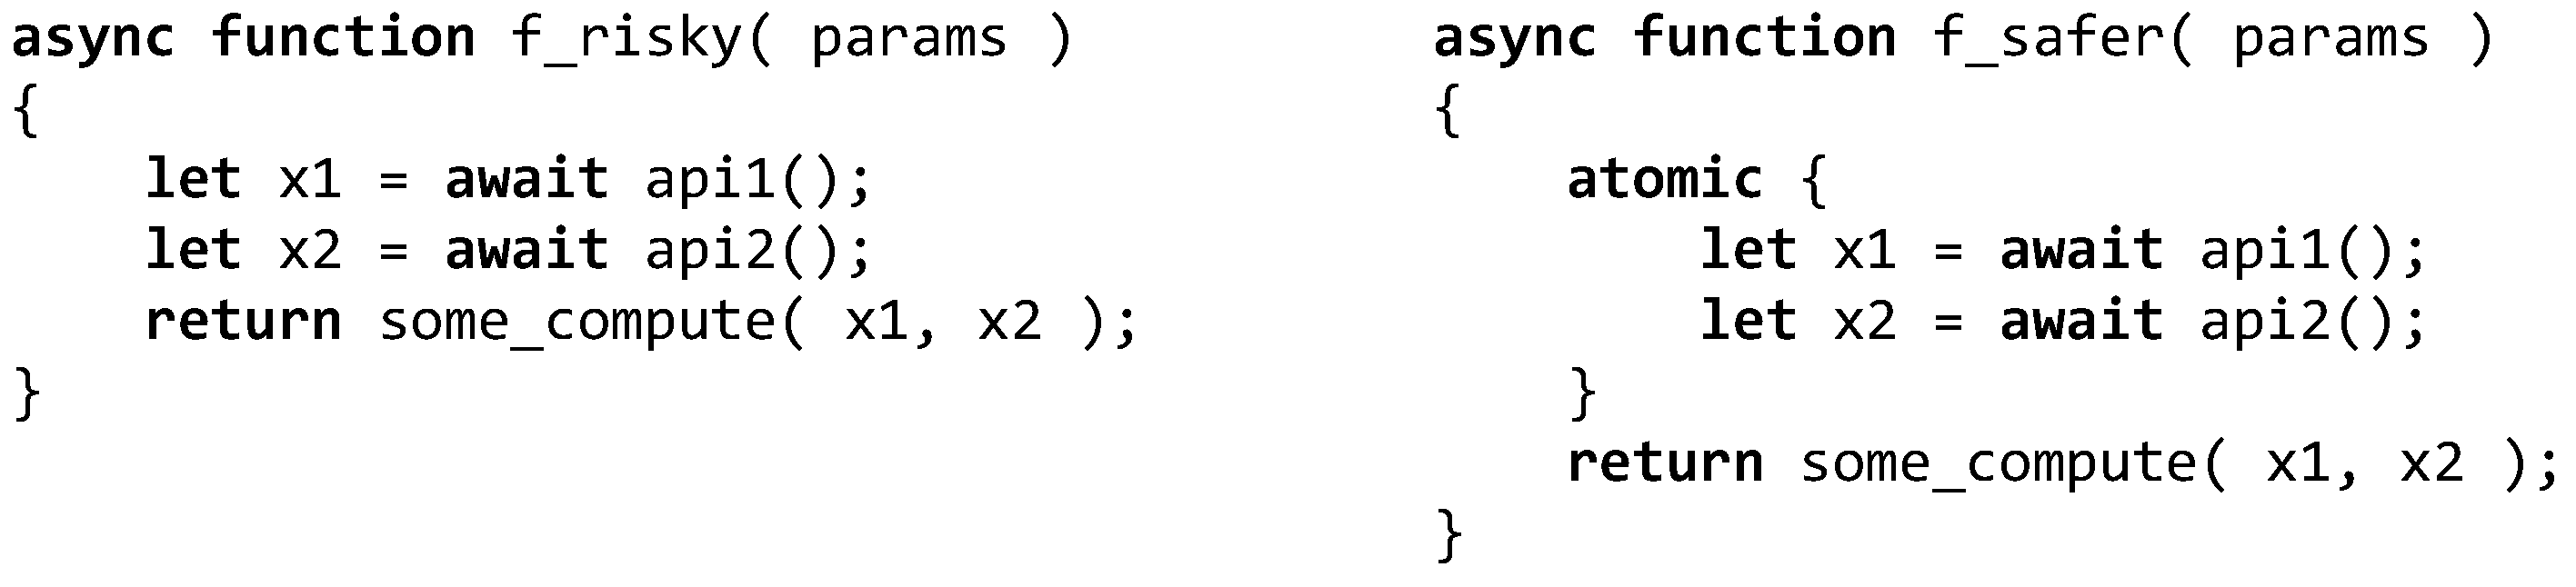
\includegraphics[width=0.9\textwidth]{Code/async_atomic_js}
\caption{A simple sketch of code that could lead to the risky gaps, and a version with an atomic block to eliminate the risk of an atomicity violation.}
\label{fig:async_atomic_js}
\end{figure}

As discussed in the previous section, there are multiple viable strategies for mitigating atomicity violation risk created by short-duration chains of continuations.
In this section we explore one of those strategies: adding an atomic block to languages like JavaScript that use event loops, coroutines or similar anonymous multitasking frameworks.
Figure \ref{fig:async_atomic_js} shows a simple sketch of how atomicity violations can arise, and our proposed solution.
Previous research has shown that atomic blocks can be an effective concurrency control mechanism in the multithreading context \cite{Pankratius2011, Pankratius2014}.
Most importantly for this project, atomic blocks are simpler to use than some alternatives (e.g. explicit mutex locks), and therefore are useful to a wider range of developers.

In this section we show that the combination of anonymous multitasking (e.g. with event loops or coroutines) and atomic blocks is problematic.

\subsubsection{Quick Aside on Preemptive, Atomic and Cooperative}

The very modest ``real world'' use of atomic in the context of preemptive multithreading languages could be seen as evidence against its usefulness in general.
One issue to consider is that in the preemptive context, implementing atomic efficiently, and cleanly defining how code running in atomic mode should interact with concurrent non-atomic code are both substantial challenges.
It seems likely that these issues have dampened enthusiasm for this feature.
For most intents and purposes, these challenges do not exist in the cooperative context.

There are a few research projects that have attempted to blur the line between preemptive and cooperative multithreading in one way or another \cite{ONeill2015, Boussinot2006, Dabrowski2006}.
The authors of this paper see the primary goals of cooperative vs preemptive multithreading to be mostly different (multitasking vs parallelism), so this blurring does not seem compelling to us.

\subsection{A Candidate Definition of Atomic for Event Loops} \label{sec:candidate_atomic}

One reasonable definition of atomic in event systems is as follows:

% \cite{Loring2017} Semantics of Asynchronous JavaScript

\begin{enumerate}
\item When some code enters an atomic block, all pending events are removed from the dispatcher and pushed collectively onto a stack of pending events.
\item The body of the atomic block runs as usual, possibly registering new events.
\item When the body of the atomic block finishes, it pauses to allow other continuations to run (i.e. the events registered by the atomic block itself).
\item Events are executed as usual (with continuations potentially registering new events).
\item Once the event dispatcher is empty, the code that was waiting at the end of the atomic block can continue; simultaneously the events that were pushed in step 1 are popped and restored to the dispatcher.
\end{enumerate}

Notice that this definition works for nested atomic blocks.
In cases where the body of an atomic block consists of a short linear chain of continuations, this definition would produce exactly the expected effect: the chain would run with no possibility of interruption.
It is when there is branching within an atomic block that the desired semantics get less clear.
Because it is not possible to distinguish between logically continuing the current task and spawning a new one, this definition effectively assumes that \emph{all} continuations are part of their parent's task, and assumes they should all be contained within the atomic block.

\subsection{Background on Nested Atomics and Spawns}

In this subsection we give a brief review of research on atomic blocks in the context of multithreading and transactional memory.
We will relate this back to event loop systems below.
The tricky semantic issue is how to define thread spawns nested within atomic blocks (and potential further nesting of both).
One good treatment of the formal semantics of this issue is \cite{Moore2008}.
Some of the possibilities that have been explored are:
\begin{itemize}
\item Spawning a thread within an atomic block is an error (static or dynamic). (\emph{spawn-error})
\item Spawns within atomic blocks are delayed until after the block has completed. (\emph{delay-spawn})
\item Threads spawned within an atomic block are allowed to run concurrently, and the block is not complete until such threads are finished. (\emph{spawn-contained})
\item Threads spawned within an atomic block are allowed to run concurrently, and are completely disconnected from the block. (\emph{spawn-unconstrained})
\end{itemize}

Unfortunately, it seems that no simple definition works well in all cases.

\emph{Spawn-error} is tempting, since it somehow feels like spawning new tasks is not in the spirit of ``atomic''.
However, this is hard to defend in practice, because there are perfectly reasonable programs that have spawns inside atomic blocks.
Consider a library function that spawns a new task.
\emph{Spawn-error} would make it impossible to wrap a call to such a function in atomic.
Furthermore, as we will see in the empirical analysis below, programs that seem to have this shape are fairly common.

The \emph{delay-spawn} strategy causes deadlock for code that spawns a short-lived task then waits for it to finish, while still in the atomic block.

The \emph{spawn-contained} strategy causes unresponsiveness for code that spawns long-lived tasks, because according to this strategy the atomic block is not finished until all spawned tasks are finished.
This is effectively the strategy enforced by the candidate definition in \textsection\ref{sec:candidate_atomic}.

%% A quick example of when the \emph{spawn-contained} policy is problematic:
%% Consider a function that performs a few quick database queries and then sends a potentially slow network request based on the results of the queries.
%% A caller may want to enforce atomicity among the database queries, but wrapping a call to this function in atomic would cause the application to become unresponsive until the network request completed.

\subsection{Do Programs Actually Do this Weird Stuff?}

Before considering approaches to handling spawns nested inside atomics, it is useful to measure whether these patterns occur with any frequency in practice.
If spawning inside atomic blocks is rare, then simple definitions (like \emph{spawn-error}) might be viable.

We analyzed the continuation trees we collected for evidence of spawning within atomic blocks.
Obviously JavaScript lacks both explicit spawning and atomic blocks, so we are simply looking for suggestive patterns.
We take continuations with multiple children (i.e. branching) as a suggestion of spawning, and we take multiple related continuations within a small time window as a suggestion of atomicity.
Specifically, we define \emph{potentially atomic subtrees} (PASs) of a continuation tree to be those that satisfy the following conditions:

\begin{itemize}
\item \emph{Nontrivial}. At least two continuations.
\item \emph{Connected}. Not forests.
\item \emph{Time limited}. The duration from the beginning of the first continuation to the end of the last must be under some time limit.
\item \emph{Maximal}. Proper subtrees of trees that satisfy these conditions do not count.
\item \emph{No Recurring}. Recurring edges are ignored, except for a special case described below.
\end{itemize}

We examined all the PASs in our data set, and found the following shapes.
For some shapes we defined variants of the criteria that we call ``looser'' or ``stricter''.

\begin{itemize}
\item \emph{Linear}. All continuations have at most one child.
  Stricter version: all children are considered.
  Looser version: recurring children do not count.
\item \emph{Multiple long-lived branches}. Looser version: Has at least two children outside the subtree (can have the same parent).
Stricter version: Has at least two children outside the subtree with different parents.
\item \emph{Contained branch}. Looser version: Has at least one continuation with no children, and at least one continuation with at least one child outside the subtree.
  Stricter version: Same as the loose version, with the additional constraint that there be at least one continuation in the subtree after the one with no children.
\end{itemize}

\begin{table}
  \centering
  \begin{tabular}{|r|r|r|r|r|r|r|}
    \hline
    Limit (ms) &  Total & Linear & Multi L & Multi S & Contain L & Contain S \\
    \hline
    1          &    837 &   66\% &    17\% &   0.7\% &      18\% &     0.2\% \\
    \hline
    10         & 17,885 &   80\% &   4.4\% &   2.1\% &      15\% &     1.3\% \\
    \hline
    100        & 46,515 &   87\% &   3.9\% &   2.3\% &     8.3\% &     1.5\% \\
    \hline
  \end{tabular}
  \caption{XXX subtrees}
  \label{table:subtrees}
\end{table}

Table \ref{table:subtrees} shows the total number of PASs and the percentage of each shape for 5 different time limits.
The first thing to observe is that most of the subtrees are linear, but not an overwhelming majority.
This suggests that a definition of atomic blocks that handles branching poorly could create problems in practice.

A small fraction of the PASs have multiple long-lived branches.
This suggests that the simple candidate definition of atomic given in \textsection\ref{sec:candidate_atomic} (\emph{spawn-contained}) would create responsiveness problems.
Implementing any of the other strategies requires that the system be able to distinguish between spawning and continuing the parent's task.

A small fraction of the PASs have contained branches.
This suggests that the \emph{delay-spawn} strategy could create deadlock problems.
Note that even for the stricter version of the contained branch criteria, we cannot say for sure that the longer branch is waiting for the shorter branch.
If it is not waiting, then the \emph{delay-spawn} strategy could be fine.

% XXX Unlike the preemptive multithreading context, where there might be a performance benefit to letting multiple threads simultaneously execute in atomic mode, we are dealing with single-threaded multitasking here.

While further study of more application families is called for, we suggest the following guidelines based on this analysis.
\emph{If} a language designer wants to introduce an atomic block into a cooperatively concurrent system:
\begin{itemize}
\item The system should have explicit task identities.
\item \emph{Delay-spawn} is a good default strategy, because it works fine with long-lived tasks spawned inside atomic blocks and it seems that truly contained spawns that can cause deadlock are fairly rare.
  Furthermore, unlike systems like NePaLTM \cite{Volos2009}, the potential parallelism advantage of running multiple tasks ``inside'' an atomic block is not relevant.
\item There should be some mechanism for programmers to override the default for specific atomic blocks and/or specific task spawns.
\end{itemize}

\section{Cooperative Threads and Atomic Blocks for JavaScript}

In this section we discuss the first of our two implementations of cooperative threading with atomic blocks.
This version is a JavaScript library built on top of generator functions (\texttt{function*}, a.k.a. coroutines).
Researchers have explored adding atomic blocks to several \emph{preemptive} multithreading languages, at least in an experimental capacity; for example: Haskell \cite{Harris2005}, OCaml \cite{Ringenburg2005}, Java \cite{Herlihy2006}, C/C++ \cite{Ni2008}.
We do not claim any novelty with respect to the basic questions of what atomic blocks should mean.
In fact, it is much easier to implement atomic blocks in the cooperative context.
The main point we explored was how easily this idea can be integrated with popular coding patterns and legacy code.

We begin by building a flavor of async functions on top of generators; this idea is discussed in the ``Informative Desugaring'' appendix to the official proposal for async functions \cite{Terlson2016}, and has been implemented in several libraries.
The main trick is a stepper process that iteratively calls the \texttt{next} or \texttt{throw} method on the generator until it is done.
Typically this stepper process is a recursive Promise chain; our library uses a standard async function for convenience.
The two differences between standard async functions and our variant (which we call \emph{\asyncs{}}) is that ours support an explicit notion of tasks, and atomic blocks.

\begin{figure}
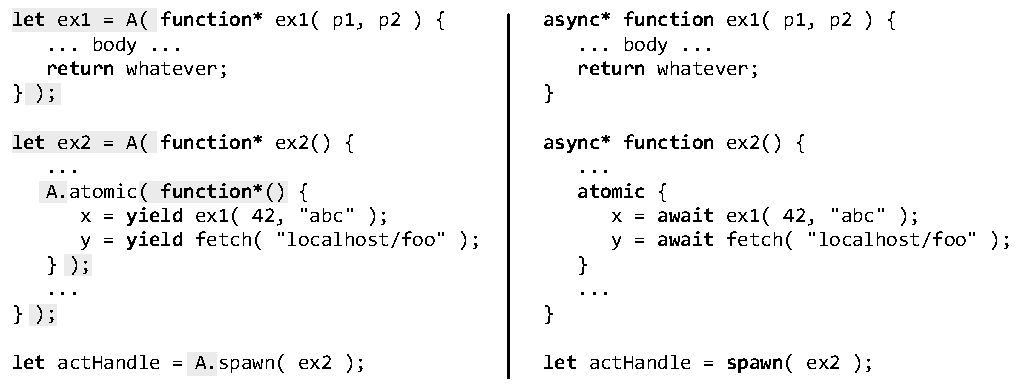
\includegraphics[scale=0.75]{Code/trivial_js}
\caption{A sketch of how our JavaScript library is used, compared to what it would look like with native syntax.
  The syntactic overhead (highlighted with a gray background) is modest.}
\label{fig:trivial_js}
\end{figure}

Implementing explicit tasks requires that a call to an \asyncs{} function ``know'' what task it belongs to.
We explored two solutions to this problem.
The first requires user code to explicitly pass an additional context parameter to all \asyncs{} functions.
This version is nicely explicit, but introduces substantial syntactic overhead and gives application code the opportunity to pass this parameter incorrectly.
The second implementation uses a global variable to implicitly pass the task context to functions that need it.
The stepper process sets this global variable to the correct task context just before taking the next step.
Figure \ref{fig:trivial_js} gives a flavor of what programming with our library looks like; notice that the syntactic overhead is modest.
A third option that we \emph{did not} explore is to use the new metaprogramming facilities in JavaScript to modify definitions of and calls to \asyncs{} functions to explicitly pass a task context parameter.

Our \asyncs{} functions mostly integrate well with legacy code.
\asyncs{} functions can await Promises, just like in standard async functions (and many callback-based functions can be trivially converted to Promise-based with the popular \texttt{promisify} library).
\asyncs{} functions can be called like regular async functions by legacy code.
However, legacy code obviously does not know about task contexts, so legacy code calling \asyncs{} functions or other functions provided by our library can result in unexpected results with respect to what task a call ``belongs'' to.
We consider such calls to be unsupported behavior.

We implement atomic by checking in each step of the stepper process whether the current task is blocked.
If it is, it adds itself to a waiting set and blocks until the relevant atomic block ends.
A consequence of this approach is that our library cannot enforce atomicity on continuations registered by legacy code.
This limitation on atomicity-enforcing power is inevitable in a library-based design.
However, if a JavaScript implementation was to adopt this design natively, it could easily enforce such atomicity in the event dispatcher.

As discussed in the previous section, what makes atomic interesting is how it interacts with task spawns.
If we assumed such nesting did not exist, \texttt{atomic} could be implemented with a single global variable that stores either the task identity of the task in atomic mode, or an empty token (i.e. \texttt{null}, or whatever).
In order to support a range of options, depending on choices made by user code, our implementation maintains a stack of \emph{atomic contexts}, which is empty when no tasks are in an atomic block.
When a task enters an atomic block, it pushes a new atomic context and saves all currently active tasks as blocked peers in that context.

By default our implementation uses the \emph{delay-spawn} strategy.
That is, newly spawned tasks are blocked and added to the peer set of the outer-most atomic-context.
To override this default, there is a variant of the spawn function that takes additional options from user code.
Currently the only implemented option is an assertion that the spawned task will be short-lived.
When short-lived tasks are spawned inside an atomic block, our implementation uses the \emph{spawn-contained} strategy, which means the atomic block does not finish until all such tasks have finished.

\subsection{Activities: A Variant of Conventional Cooperative Threads}

The design that we ended up with is mostly like conventional cooperative multithreading with an atomic block.
In this paper we do not present any formal semantics; rather, we refer to existing work on the semantics of cooperative threads \cite{Abadi2009} and atomic blocks \cite{Moore2008}.
One difference we noticed is that there is an implicit interruption point (i.e. \emph{yield}) at the end of every step of the stepper process.
Looking at this slightly differently, it can be seen as an implicit yield just before and after each call to an \asyncs{} function.
While these implicit yields arose as a side-effect of our implementation, upon further reflection, this design seems interesting in its own right.
We named these cooperative threads with implicit yields before and after non-atomic calls \emph{activities}, and we analyze their pros and cons in the next section.

\subsection{Continuation Fusion}

We briefly note an efficiency opportunity enabled by atomic blocks.
For short chains of continuations, the overhead associated with moving in and out of the event dispatcher can be nontrivial.
In a version of JavaScript with native atomic blocks, it would be possible to fuse atomic chains of continuations into a single function, eliminating this overhead.

% XXX Doppio ??? \cite{Vilk2014}



%% Acknowledgments
%% \begin{acks}                            %% acks environment is optional
%%                                         %% contents suppressed with 'anonymous'
%%   %% Commands \grantsponsor{<sponsorID>}{<name>}{<url>} and
%%   %% \grantnum[<url>]{<sponsorID>}{<number>} should be used to
%%   %% acknowledge financial support and will be used by metadata
%%   %% extraction tools.
%%   This material is based upon work supported by the
%%   \grantsponsor{GS100000001}{National Science
%%     Foundation}{http://dx.doi.org/10.13039/100000001} under Grant
%%   No.~\grantnum{GS100000001}{nnnnnnn} and Grant
%%   No.~\grantnum{GS100000001}{mmmmmmm}.  Any opinions, findings, and
%%   conclusions or recommendations expressed in this material are those
%%   of the author and do not necessarily reflect the views of the
%%   National Science Foundation.
%% \end{acks}




% We recommend abbrvnat bibliography style.

% \bibliographystyle{abbrvnat}
% \bibliographystyle{abbrv}

% The bibliography should be embedded for final submission.

\bibliography{./coop_measurement.bib}

%% \begin{thebibliography}{../../../../Documents/PapersForReferencing/biy_all_research.bib}
%% \softraggedright

%% \end{thebibliography}

\end{document}
